\hypertarget{component}{}\section{Topology and Component
}\label{topology}
HSA platform topology information is provided by the runtime by way of
data structures so user can gather details about how a HSA
system/platform exposed its architectural details such as
\DIFdelbegin \DIFdel{components, memory, caches and connectivity (platform topology
requirement is described in the SAR document)}\DIFdelend \DIFaddbegin \DIFadd{agents and memory}\DIFaddend . This information
could be utilized by the user in different ways including decisions
on where to execute a particular user task. Core runtime
specification defines the topology table data structure and other
data structures to represent topology hierarchy.  After the core
runtime is initialized with \ttbf{hsa\_open}, the user may create a
local copy of the topology information using the API
\ttbf{hsa\_topology\_table\_create}. The user can parse this table
representing the HSA system to gather details such as the number of
different HSA Components on the system with local access to a
particular set of memory resources. \DIFaddbegin \DIFadd{Topology table is designed to be
allocated in a block of contiguous memory.
}\DIFaddend

The \ttbf{hsa\_topology\_table\_create} API is defined as follows:

\input{example/APItopology_create}

The API returns \dbtt{HSA\_STATUS\_SUCCESS} if the table has been
successfully created and returned by way of the {\itshape header}. Otherwise,
it returns one of the following errors:

\begin{easylist}
& \dbtt{HSA\_STATUS\_ERROR\_INVALID\_ARGUMENT} if {\itshape header}
is NULL.

& \dbtt{HSA\_STATUS\_ERROR\_OUT\_OF\_RESOURCES} if there is a failure
in allocation of an internal structure required by the core runtime
or in the creation of table header or the actual table.
\end{easylist}

\begin{figure}
  \centering
  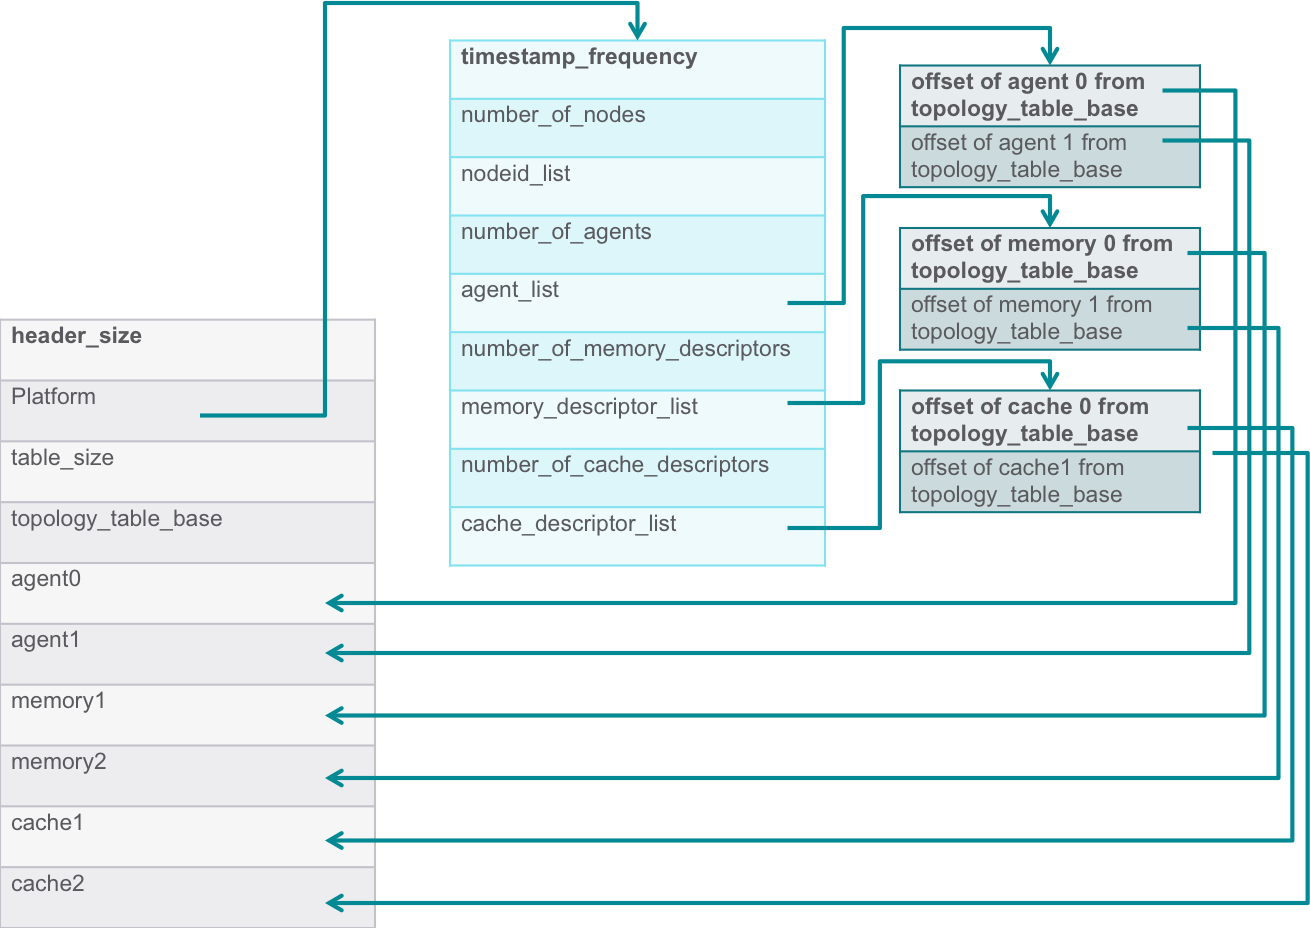
\includegraphics[width=0.5\textwidth]{fig/topologytable}
  \centering
  \caption{Structure of the Topology Table}
  \label{fig:topology_table}
\end{figure}

The table structure is shown in Figure~\ref{fig:topology_table}.
The first entity in the table is a table header. This is the output
of the \ttbf{hsa\_topology\_table\_create} API.
The table header is defined by the following structure:
\input{example/STRtopology_header}

The table header structure includes the platform structure (
\dbtt{hsa\_platform\_t}).  The platform information in the platform
structure includes size/offset-array pairs for HSA agents
(\dbtt{hsa\_agent\_t}), memory (\dbtt{hsa\_memory\_descriptor\_t}) and
cache (\dbtt{hsa\_cache\_descriptor\_t}).
HSA platform can have a hierarchical structure with multiple
components/agents and physical memories.  The
\dbtt{hsa\_platform\_t} structure also includes properties such as
the clock frequency that are common across the platform and also
links to various elements in the topology table (see Figure
\ref{fig:topology_table} ).

The platform structure is defined as follows:

\input{example/STRhsa_platform}

When no information is available for a particular element, the
corresponding {\itshape number\_ \textless element \textgreater s}
field is set to zero by the runtime in the platform structure.
Platform structure maps to the agents, cache and physical memory,
\DIFdelbegin \DIFdel{etc.}%DIFDELCMD < \, %%%
\DIFdelend in the topology table for all nodes in the platform.

The core runtime defines the following structure to represent cache:
\input{example/STRhsa_cache_descriptor}
The structure holds associativity, cache size, cache line size for
all levels of cache and the inclusive property for all but the
last level. Each cache in the HSA system has a unique cache ID
identifying it.

The memory descriptor structure represents a physical memory block
or region and includes elements to provide bandwidth \DIFaddbegin \DIFadd{(an
implementation may chose to return 0 in the }{\itshape
\DIFadd{peak}\_bandwidth\_mbps} \DIFadd{field if it cannot provide bandwidth)}\DIFaddend , interleave
characteristics and latency for accessing memory. Implementations
may choose not to provide memory bandwidth or latency information.
The memory descriptor structure is defined as follows:

\input{example/STRhsa_memory_descriptor}

The structure:
\input{example/STRhsa_segment}
can represent any combination of the 7 HSA segments, a single
bit for each segment.

The HSA Agent data structure represents an HSA component when the
{\itshape agent\_type} field in the agent structure is set to a 1
(i.e. bit 0 is set to 1).
The structure contains elements that describe its properties. Each
component has access to coherent global memory (the HSA global
segment, and as per the requirement defined in SAR, has access to
other segments as well). The {\itshape agent\_type} is utilized as a
bit-field. Setting bit 2 indicates that the agent is a host, bit 3
indicates that agent can participate in agent dispatches. All
three bits or a combination of them can be set by the HSA runtime.

The structure of the HSA agent/component is defined as follows:
\input{example/STRhsa_component}

Within the agent, the agent type is an enumeration that is defined
as follows:
\input{example/ENUagent_type}

The user must destroy the topology table before closing the runtime.
The \dbtt{hsa\_topology\_table\_destroy} API is defined by the
runtime for the user to destroy the topology table. Once a table is
created, some parts of it may become invalid if any HW is
hot-plugged/unplugged or encounters an error. If such a change
occurs, the HSA runtime generates an asynchronous error (see
Section~\ref{asyncerror}) with the \dbtt{hsa\_status\_t} enumeration
of \dbtt{HSA\_ERROR\_TOPOLOGY\_CHANGE}. This is an indication to the
user that any current usage of topology table must be stopped and a
new topology table obtained by using the
\ttbf{hsa\_topology\_table\_create} API call. The runtime guarantees
that any call made to \ttbf{hsa\_topology\_table\_create} API after
the asynchronous error is observed will return the latest version of
the topology table at the time of the API invocation. However, if
the same HW was hot-swapped out and in with the same interval, or if
the error encountered in a component was recovered, the topology
table may not look different from the users perception.

\hypertarget{topology_example}{} \subsection{Topology Example}
This is {\color{red} work-in-progress} -- the chapter needs to be written.
